\documentclass[11pt]{article}
\usepackage[T1]{fontenc}
\usepackage[utf8]{inputenc}
\usepackage[margin=2.5cm]{geometry}
\usepackage{booktabs}
\usepackage{graphicx}
\graphicspath{{Plots/}}
\title{DGE-METRIC Sensitivity Report\\\large Batch\_20260724\_074032}
\author{DGE-METRIC}
\date{2026-07-24}
\begin{document}
\maketitle
\section*{Run Summary}
\begin{tabular}{llrl}
\toprule
Case & Status & Duration (min) & Overrides \\
\midrule
etaQA2\_low & ok & 5.083 &  \\
etaQA2\_high & ok & 5.356 &  \\
\bottomrule
\end{tabular}
\section*{Top Parameter Impacts (terminal-year \% deviation)}
\begin{tabular}{llr}
\toprule
Parameter & Value & Deviation (\%) \\
\midrule
01\_etaQA2\_low &  & -3.432 \
02\_etaQA2\_high &  & -0.3493 \
\bottomrule
\end{tabular}
\section*{Terminal-Year Comparison (2050)}
\subsection*{Baseline}
\begin{tabular}{lrrrr}
\toprule
Case & Y\_1 & E\_1 & Q\_2\_1 & Q\_3\_1 \\
\midrule
01\_etaQA2\_low & 719.7 & 25 & 76.72 & 7110 \\
02\_etaQA2\_high & 719.7 & 25 & 76.72 & 1622 \\
\bottomrule
\end{tabular}
\subsection*{NZ}
\begin{tabular}{lrrrr}
\toprule
Case & Y\_1 & E\_1 & Q\_2\_1 & Q\_3\_1 \\
\midrule
01\_etaQA2\_low & 695 & 5 & 15.34 & 1.066e+04 \\
02\_etaQA2\_high & 717.2 & 5 & 15.34 & 2427 \\
\bottomrule
\end{tabular}
\subsection*{NZ\_minus\_Baseline}
\begin{tabular}{lrrrr}
\toprule
Case & Y\_1 & E\_1 & Q\_2\_1 & Q\_3\_1 \\
\midrule
01\_etaQA2\_low & -24.7 & -20 & -61.37 & 3545 \\
02\_etaQA2\_high & -2.513 & -20 & -61.37 & 804.4 \\
\bottomrule
\end{tabular}
\section*{Selected Trajectories}
\begin{figure}[h!]
\centering
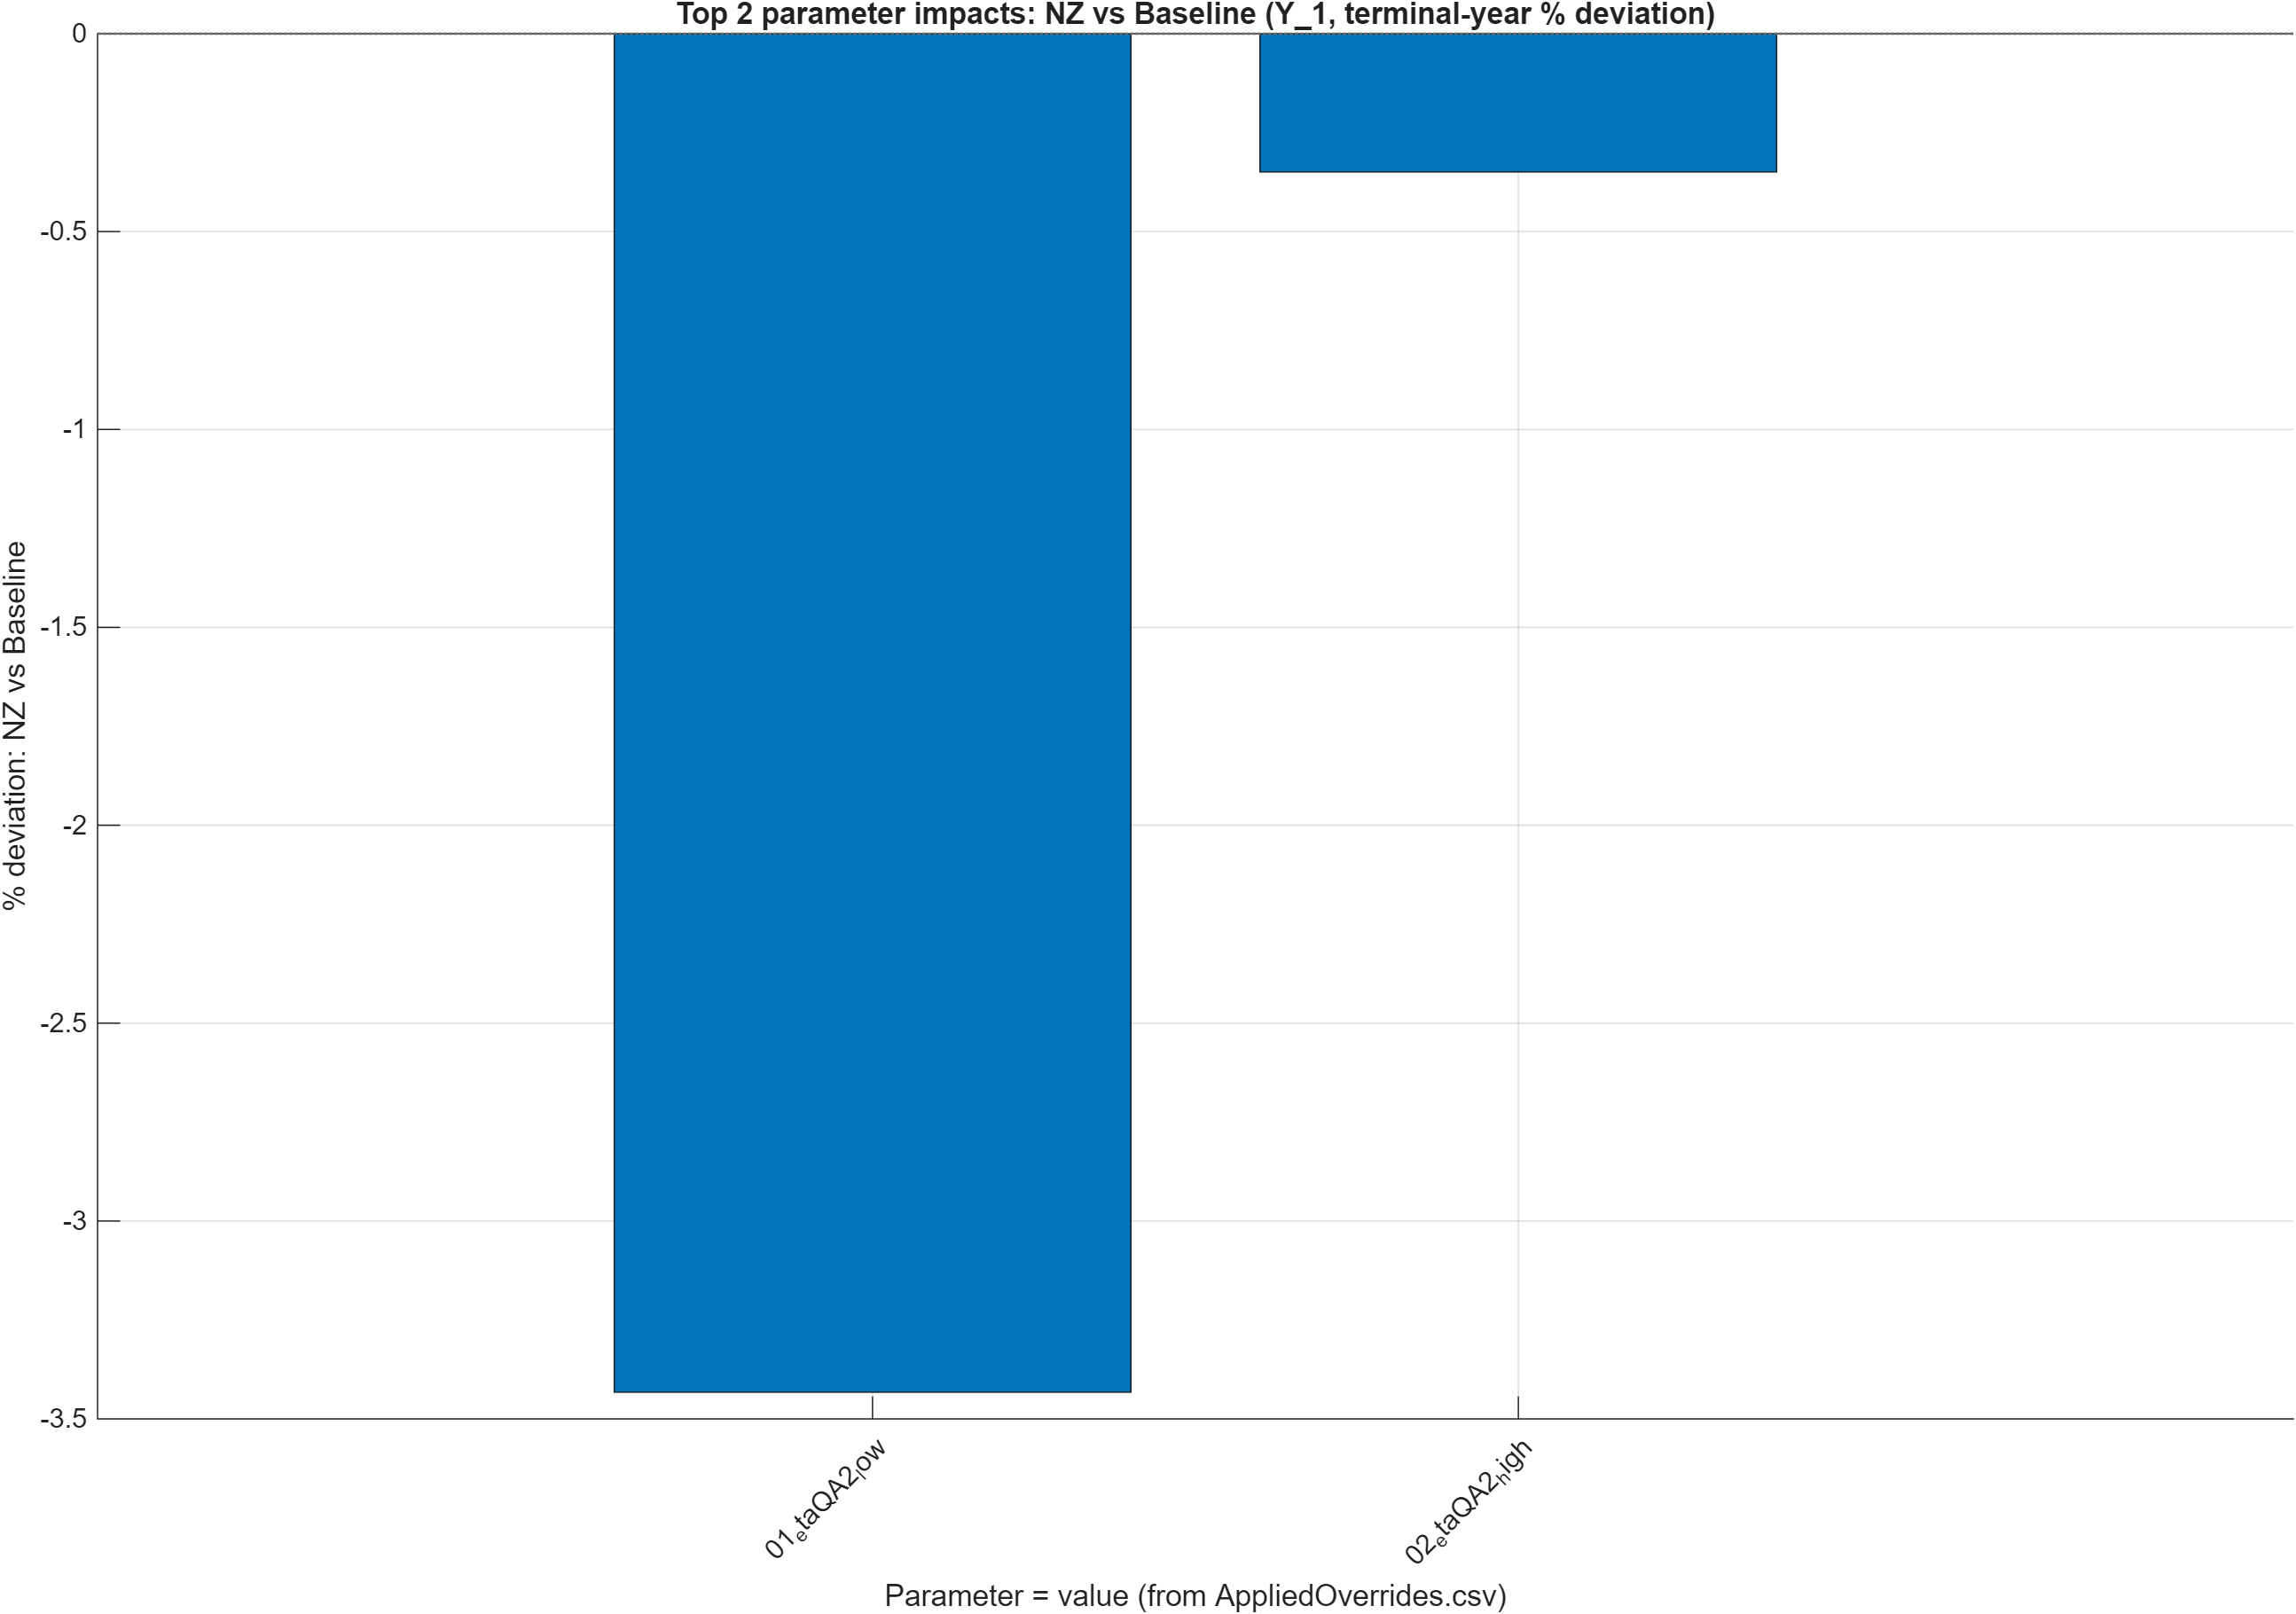
\includegraphics[width=0.85\linewidth]{ImpactTop2__NZ_vs_Baseline__Y_1.png}
\caption{ImpactTop2 | NZ\_vs\_Baseline | Y\_1}
\end{figure}
\begin{figure}[h!]
\centering
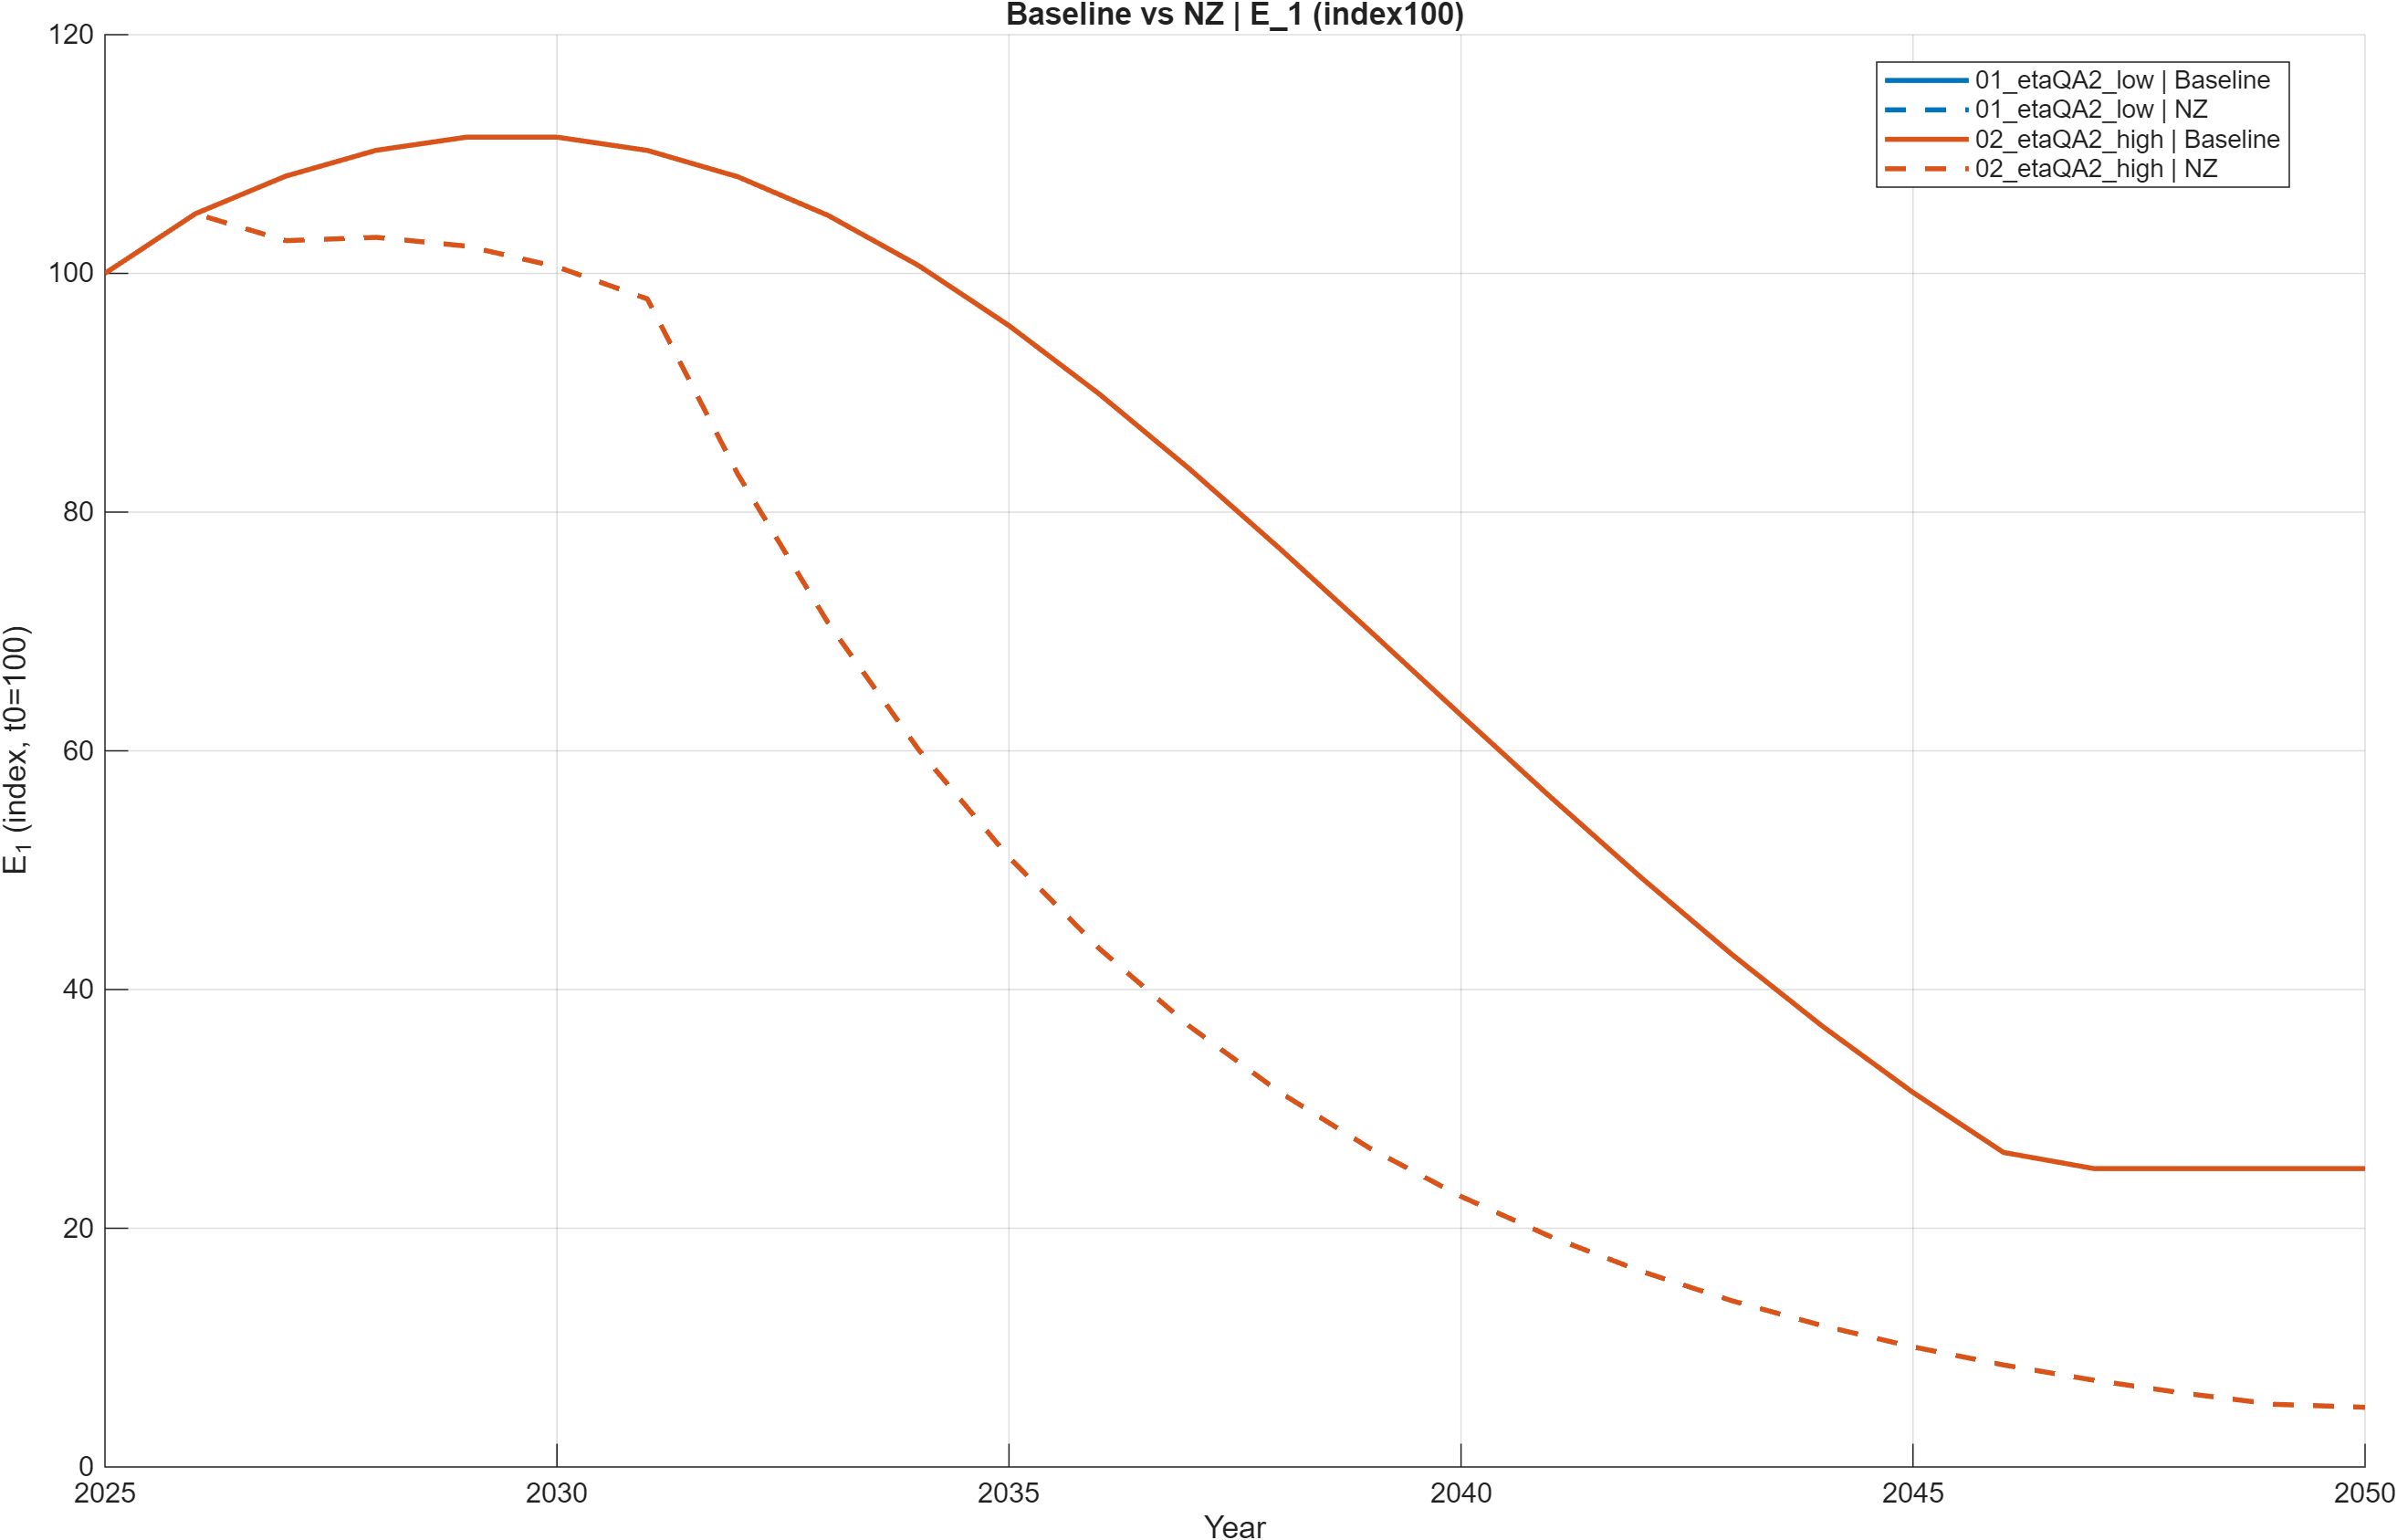
\includegraphics[width=0.85\linewidth]{Comparison__Baseline_vs_NZ__E_1__index100.png}
\caption{Comparison | Baseline\_vs\_NZ | E\_1 | index100}
\end{figure}
\begin{figure}[h!]
\centering
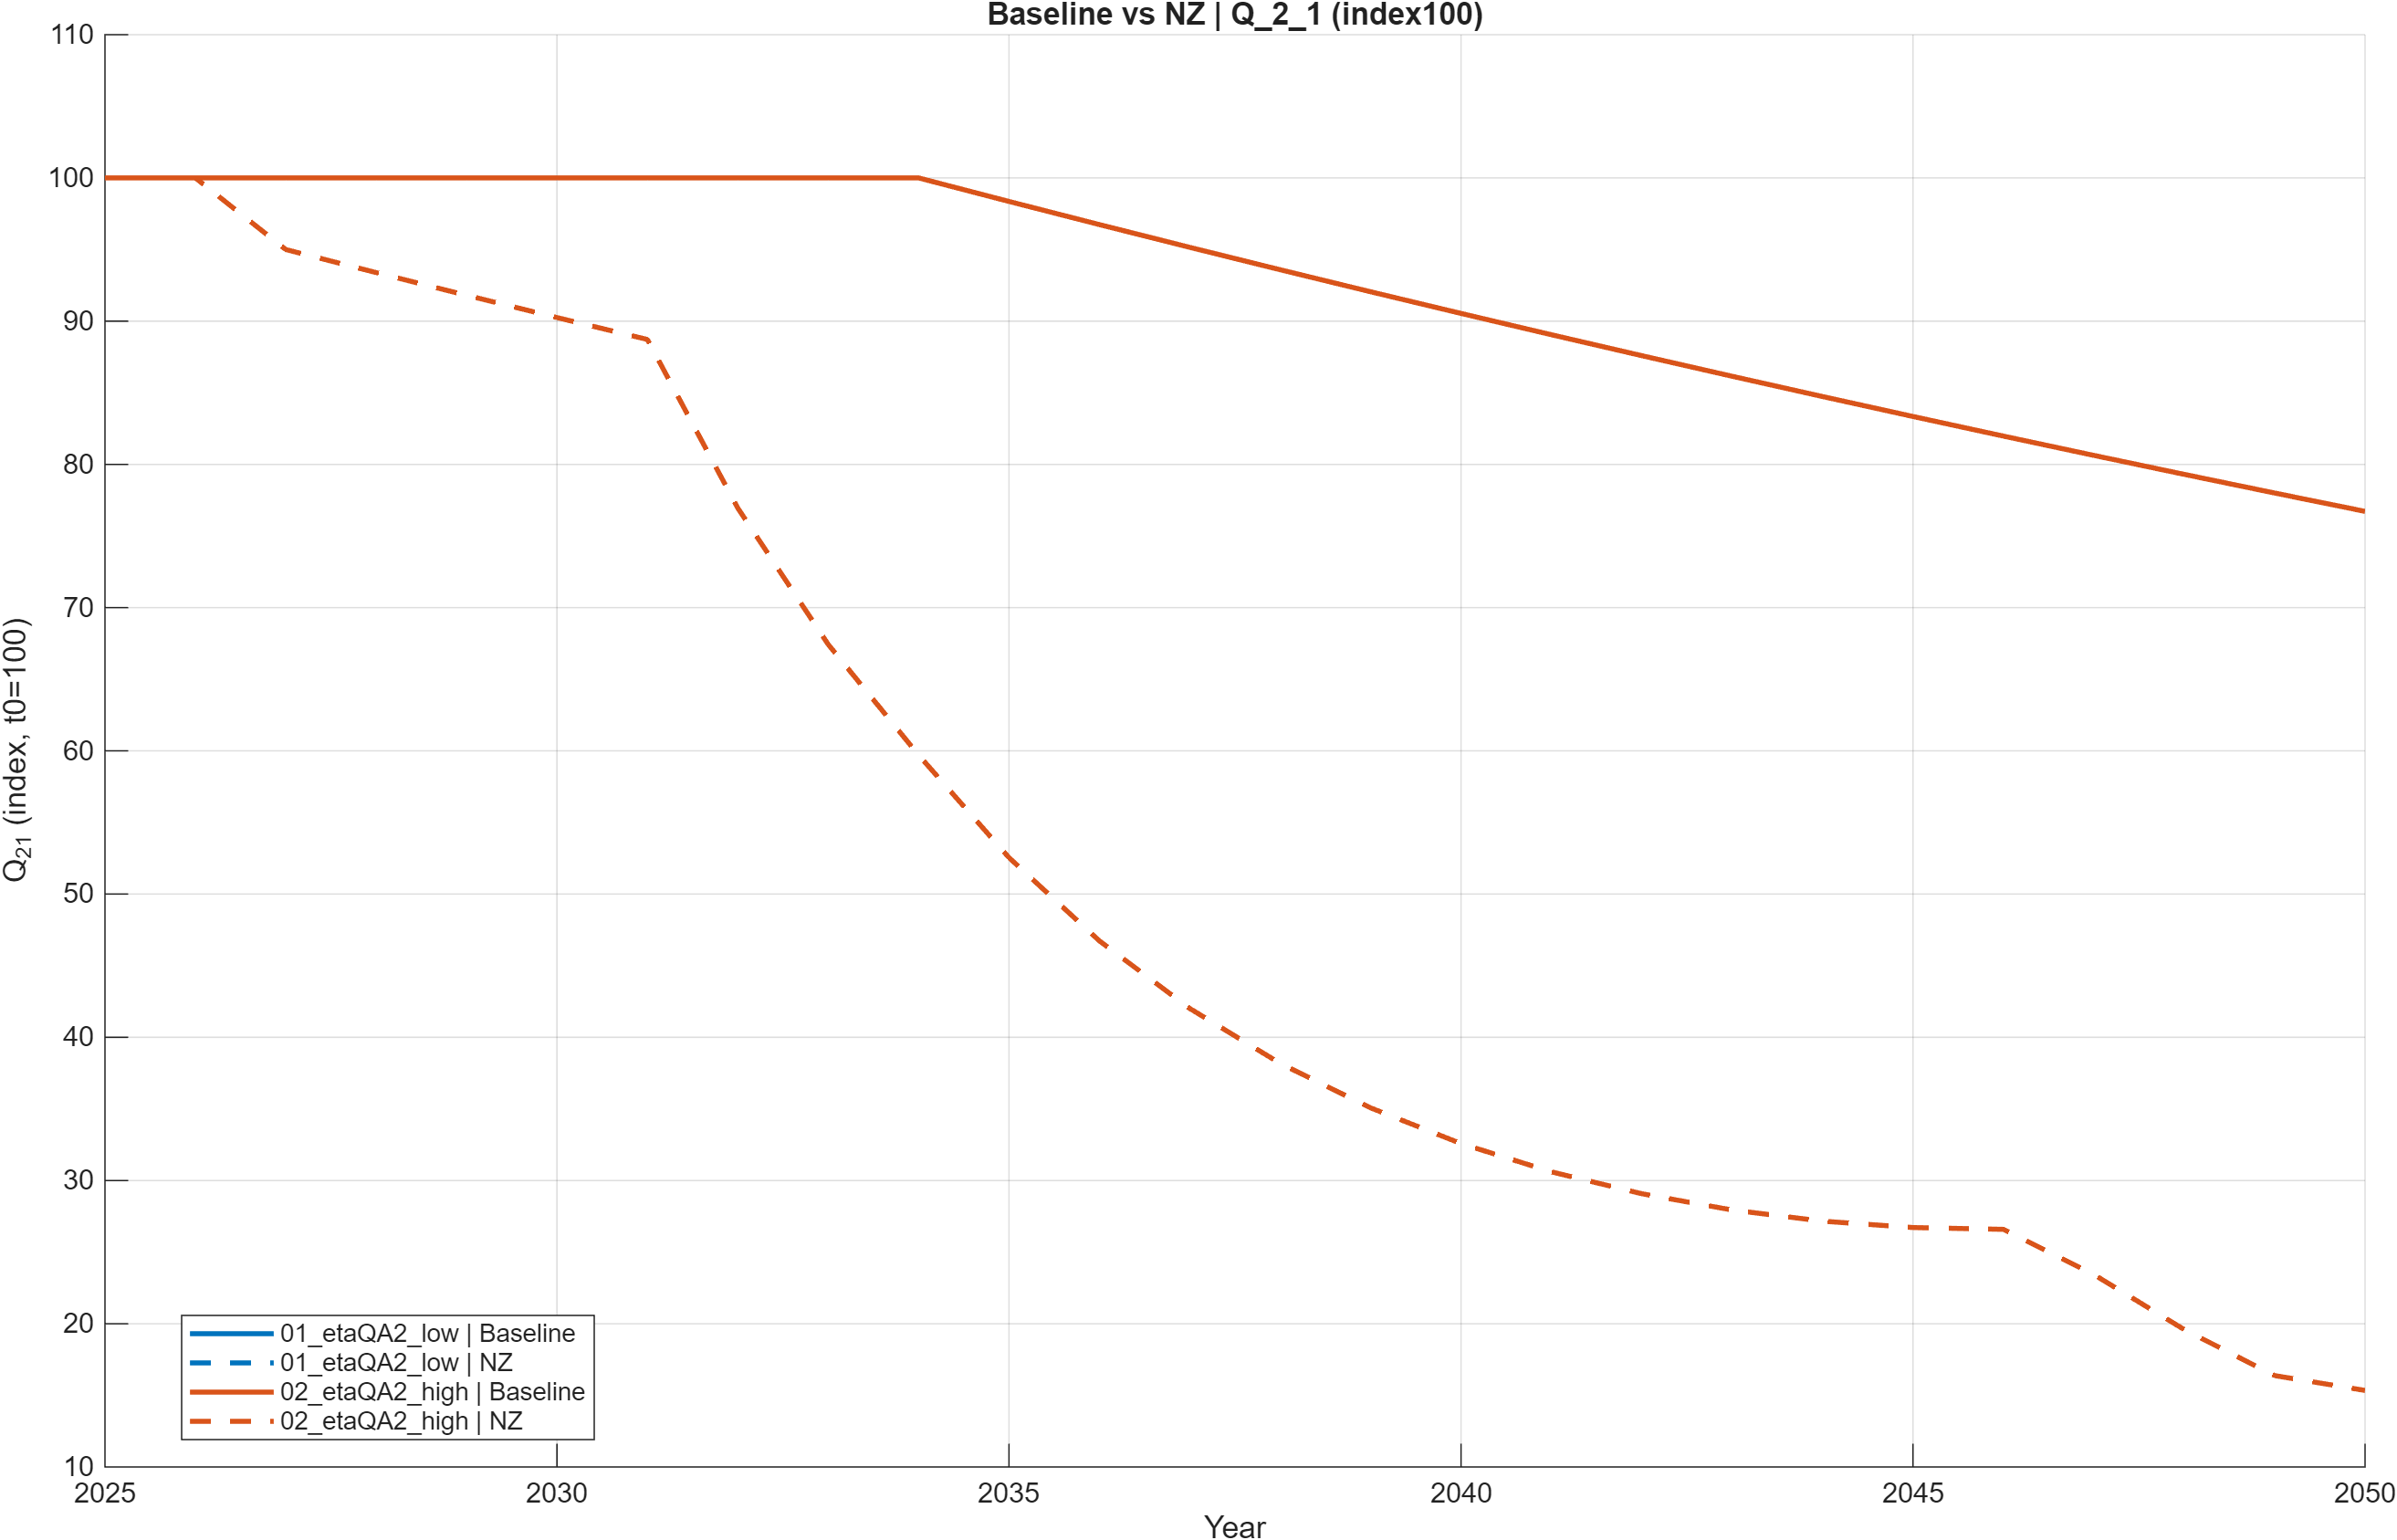
\includegraphics[width=0.85\linewidth]{Comparison__Baseline_vs_NZ__Q_2_1__index100.png}
\caption{Comparison | Baseline\_vs\_NZ | Q\_2\_1 | index100}
\end{figure}
\begin{figure}[h!]
\centering
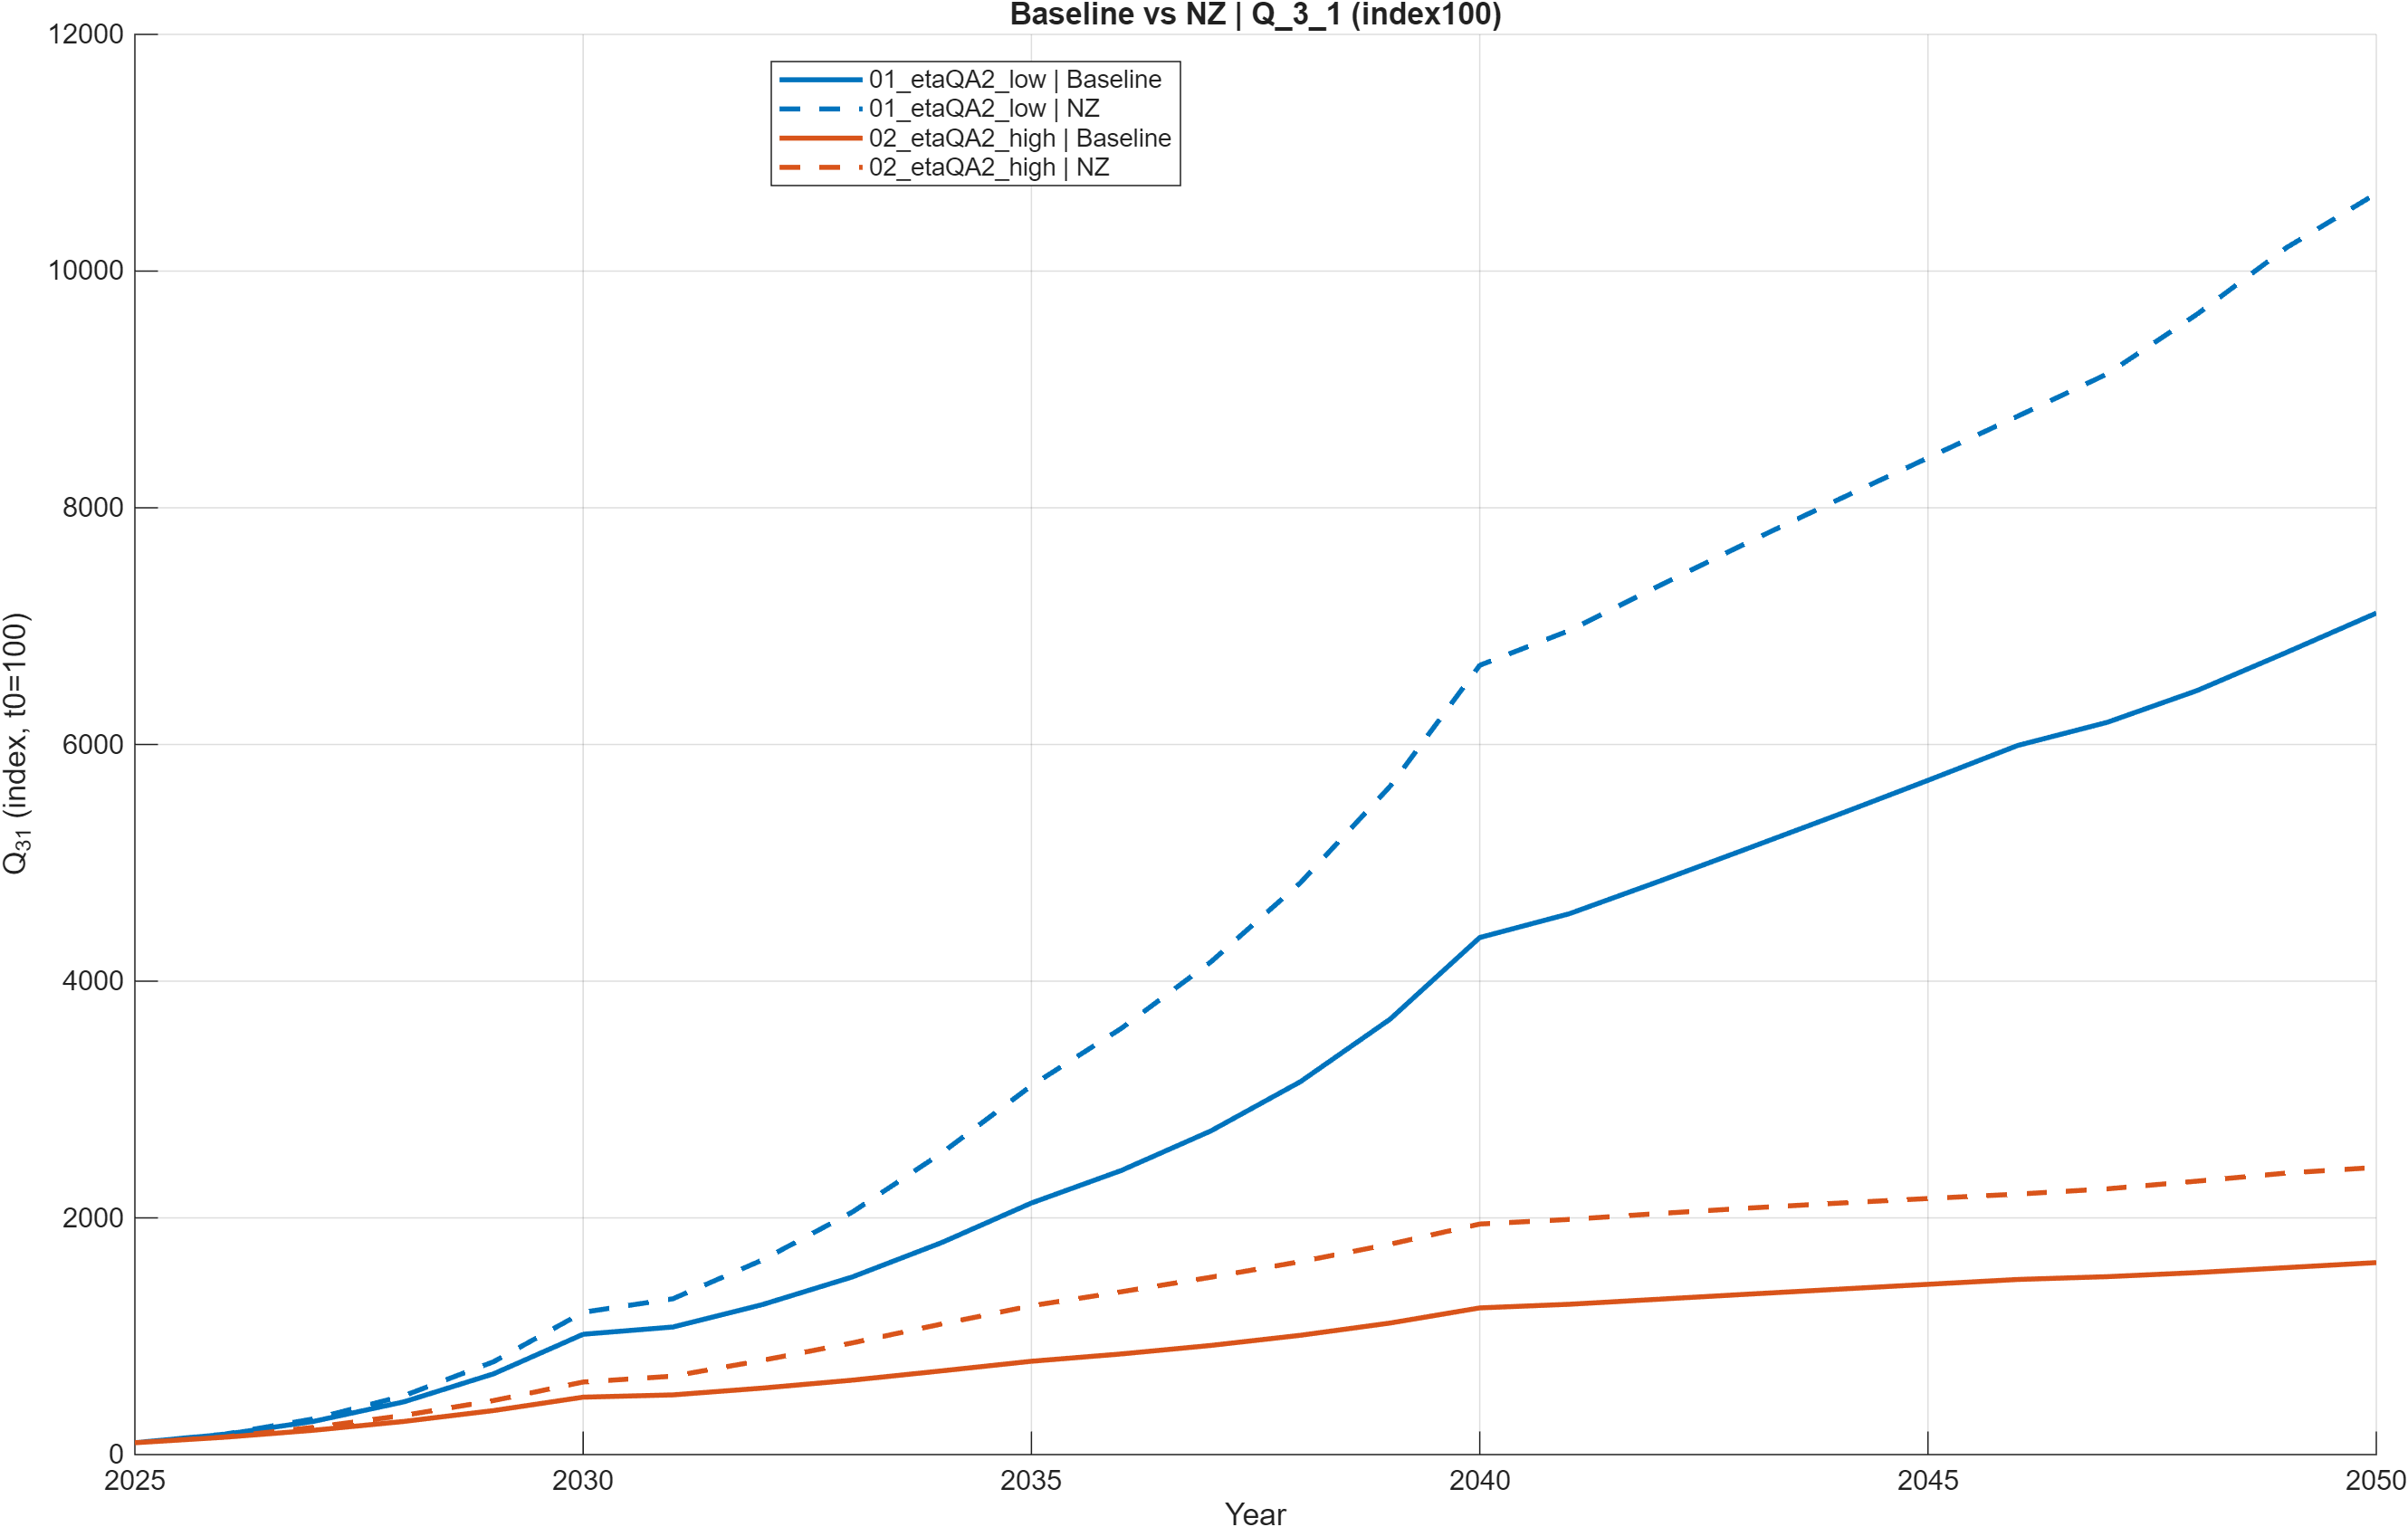
\includegraphics[width=0.85\linewidth]{Comparison__Baseline_vs_NZ__Q_3_1__index100.png}
\caption{Comparison | Baseline\_vs\_NZ | Q\_3\_1 | index100}
\end{figure}
\begin{figure}[h!]
\centering
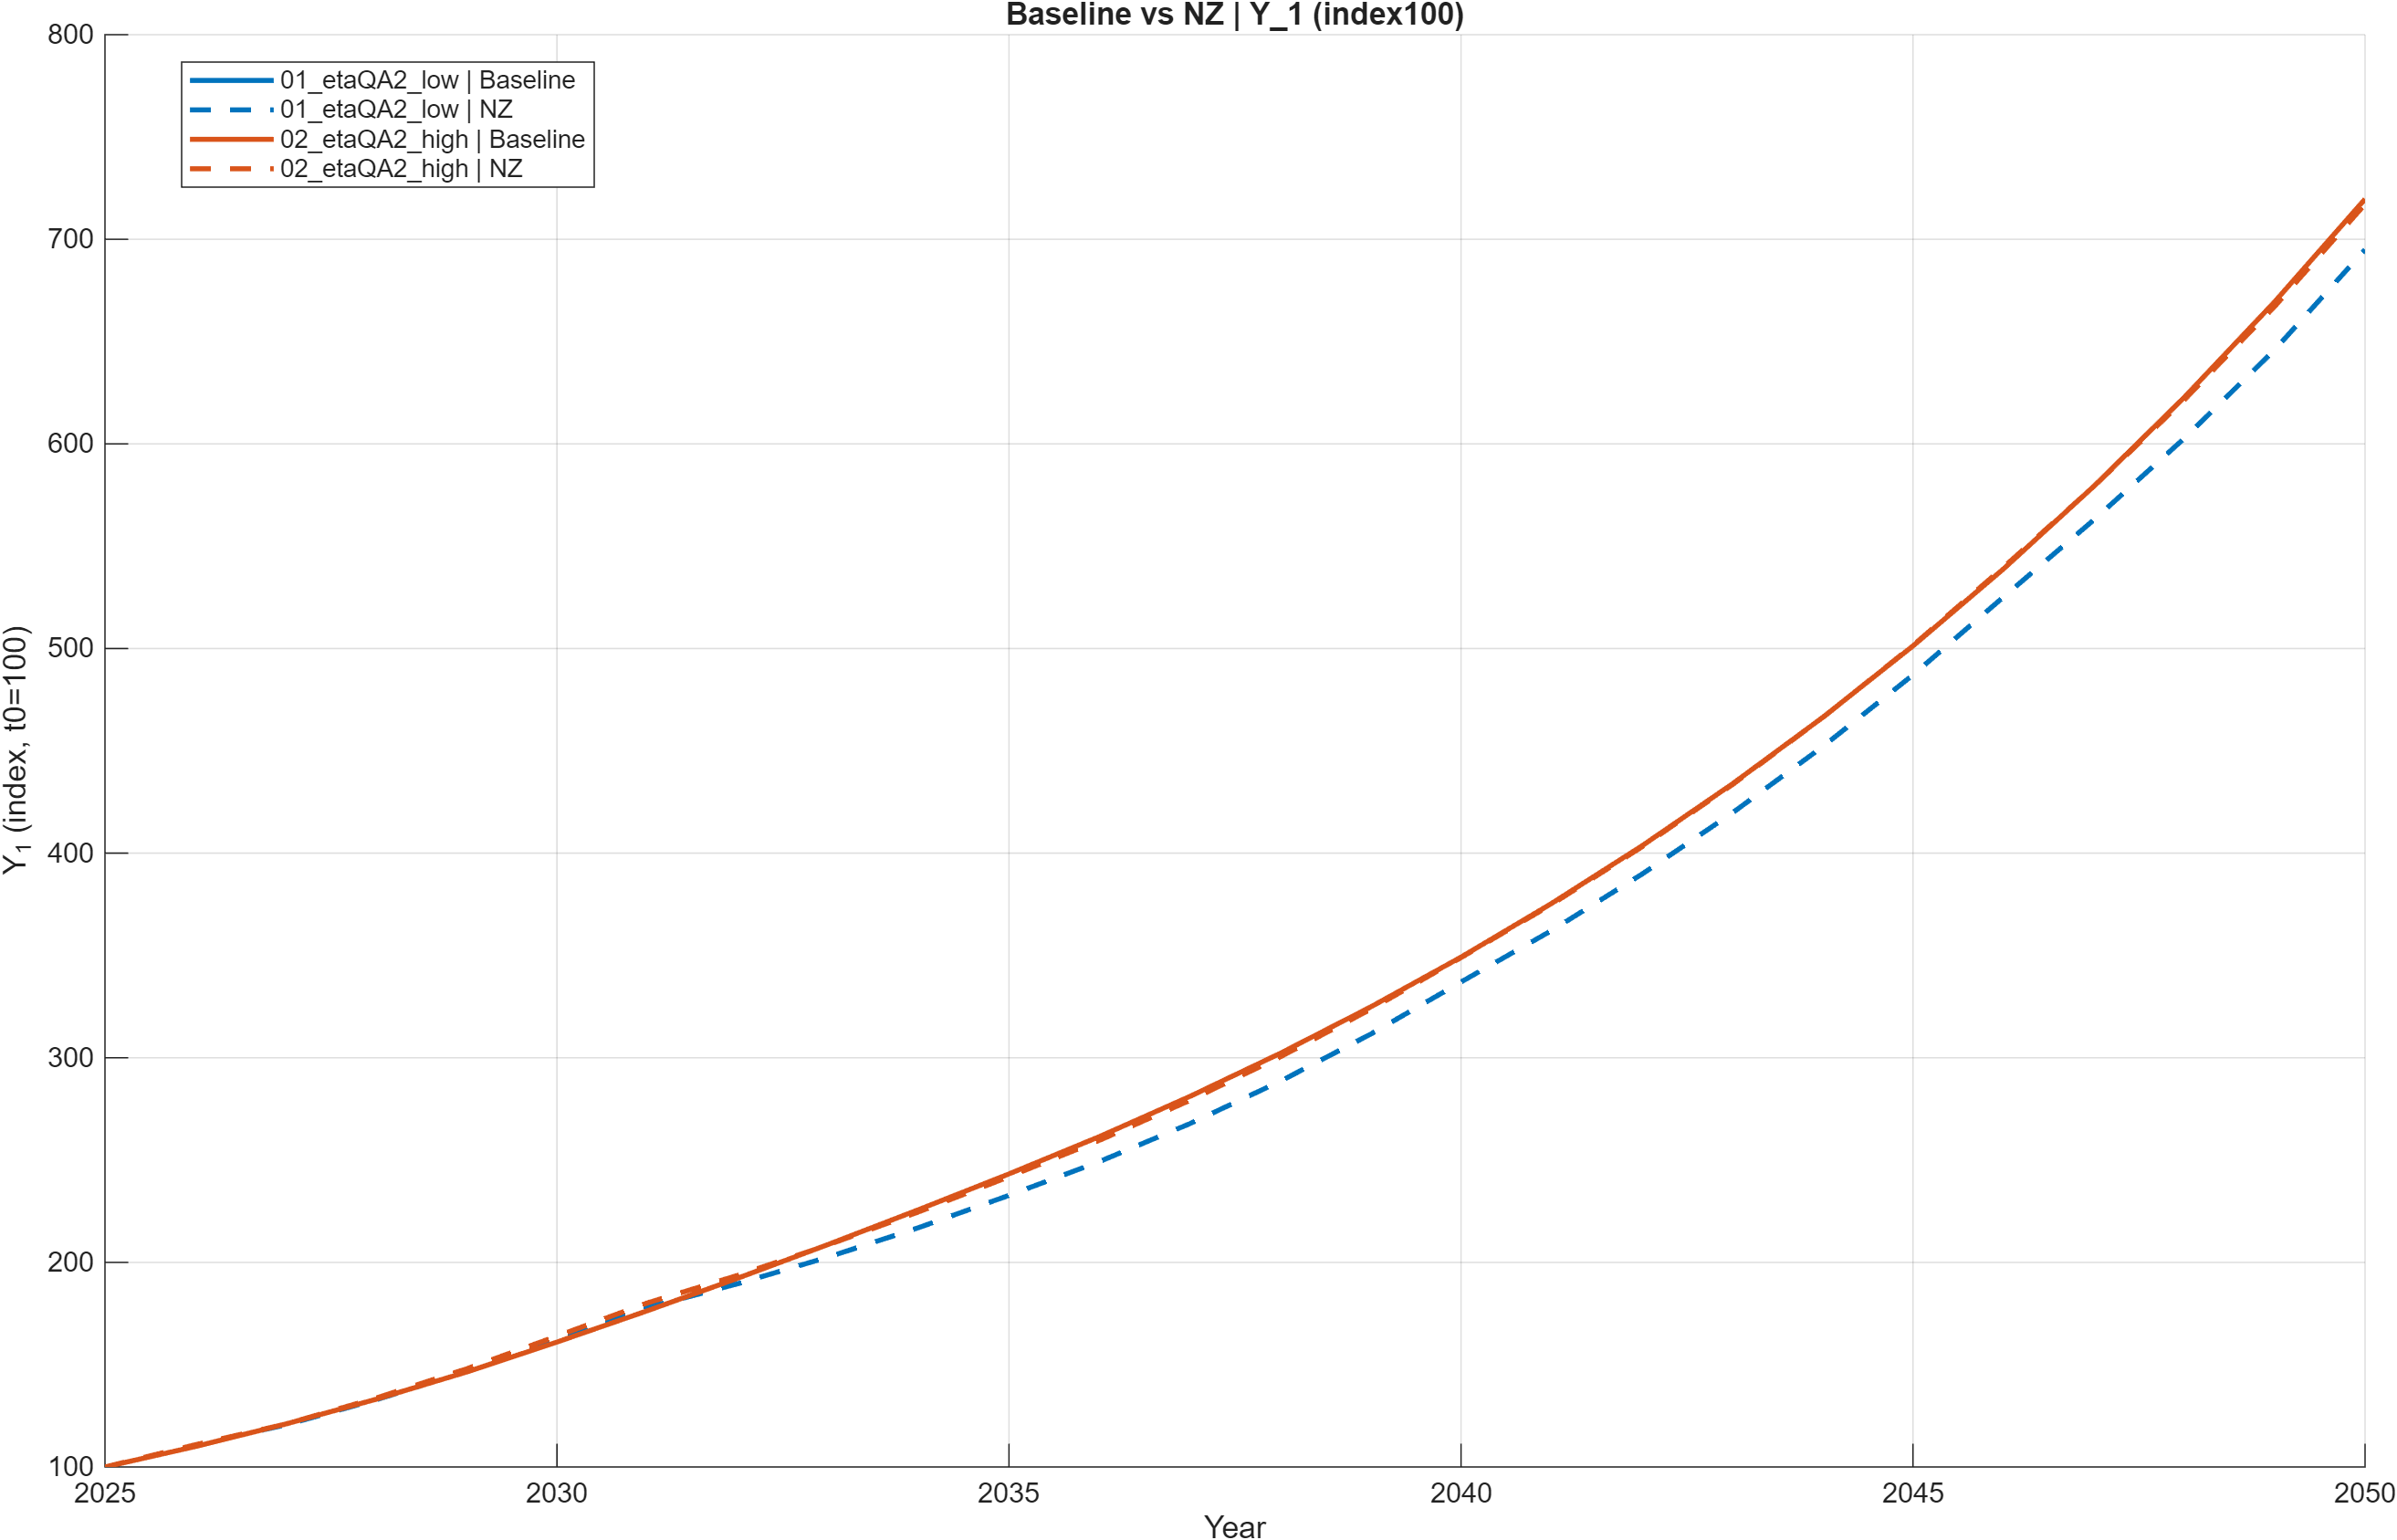
\includegraphics[width=0.85\linewidth]{Comparison__Baseline_vs_NZ__Y_1__index100.png}
\caption{Comparison | Baseline\_vs\_NZ | Y\_1 | index100}
\end{figure}
\end{document}
